% ----------------------------------------------------------------------------------------\
% ---------------------------------------------------------------------------------------\
% --------------------------------------------------------------------------------------\
\section{Análisis e interpretación de resultados}
% ----------------------------------------------------------------------------------------\
% ---------------------------------------------------------------------------------------\
% --------------------------------------------------------------------------------------\


\subsection{Código}

Este es el código usado para imprimir la matriz, se uso en cada uno del los modelos para 
ver de mejor manera esta información.

\begin{lstlisting}[style=mystylepython, language=Python, caption= código de grafico de matriz]
    plt.figure(figsize=(8, 6))
    sns.heatmap(nombre_modelo, annot=True, fmt='d', cmap='Blues', cbar=False)
    plt.xlabel('Prediccion ')
    plt.ylabel('Valor Real')
    plt.title('Matriz de Confusion para <nombre modelo>')
    plt.show()    
\end{lstlisting}

% ----------------------------------------------------------------------------------------\
% ---------------------------------------------------------------------------------------\
\subsection{Logistic Regression}
% ----------------------------------------------------------------------------------------\
% ---------------------------------------------------------------------------------------\

\subsubsection*{Métricas de evaluación}

\begin{itemize}
    \item Precisión: para la clase ham es del $91\%$, este es el porcentaje de los mensajes clasificados como ham fueron realmente ham.
    \item Recall: para la clase ham es del $92\%$, es decir el modelo identificó correctamente el $92\%$ de todos los mensajes ham.
    \item F1-score: para ambas clases (ham y spam) se obtuvo un equilibrio del $91\%$.     
    \item Accuracy: La exactitud general del modelo es del $91\%$.
\end{itemize}


\subsubsection*{Matriz de confusión}

\begin{center}
    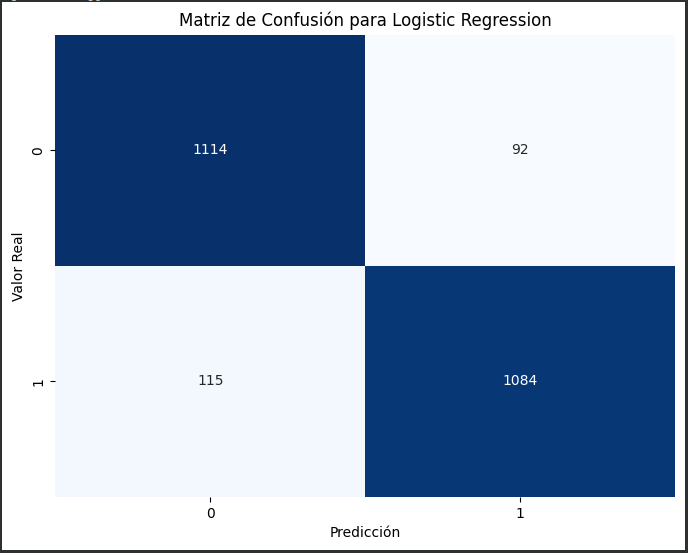
\includegraphics[scale = .4]{IMA/LogisticRegressionMatriz.png}
\end{center}

\begin{itemize}
    \item Verdaderos positivos (TP): 1114 (mensajes 'ham' clasificados correctamente como 'ham').
    \item Falsos positivos (FP): 92 (mensajes 'spam' clasificados incorrectamente como 'ham').
    \item Falsos negativos (FN): 115 (mensajes 'ham' clasificados incorrectamente como 'spam').
    \item Verdaderos negativos (TN): 1084 (mensajes 'spam' clasificados correctamente como 'spam').
\end{itemize}

% ----------------------------------------------------------------------------------------\
% ---------------------------------------------------------------------------------------\
\subsection{Support Vector Machine }
% ----------------------------------------------------------------------------------------\
% ---------------------------------------------------------------------------------------\

\subsubsection*{Métricas de evaluación}

\begin{itemize}
\item Precisión: para la clase 'ham' es del $93.43\%$, es decir ese porcentaje de mensajes clasificados como 'ham' fueron realmente 'ham'
\item Recall: identificó correctamente el $95\%$ de todos los mensajes 'ham'
\item F1-score: para ambas clases (ham y spam) se obtuvo un equilibrio del $93\%$.
\item Accuracy: La exactitud general del modelo es del $93\%$.
\end{itemize}

\subsubsection*{Matriz de confusión}

\begin{center}
    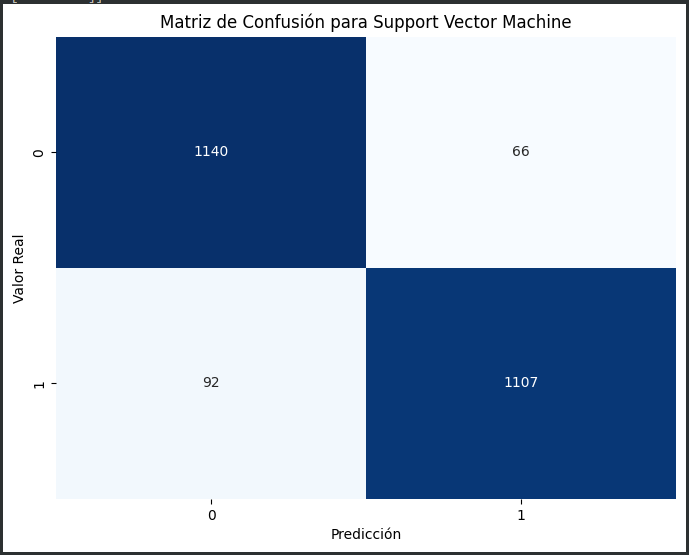
\includegraphics[scale = .4]{IMA/SupportVectorMachineMatriz.png}
\end{center}

\begin{itemize}
\item Verdaderos positivos (TP): 1140 (mensajes 'ham' clasificados correctamente como 'ham').
\item Falsos positivos (FP): 66 (mensajes 'spam' clasificados incorrectamente como 'ham').
\item Falsos negativos (FN): 92 (mensajes 'ham' clasificados incorrectamente como 'spam')
\item Verdaderos negativos (TN): 1107 (mensajes 'spam' clasificados correctamente como 'spam')
\end{itemize}

% ----------------------------------------------------------------------------------------\
% ---------------------------------------------------------------------------------------\
\subsection{Decision Tree}
% ----------------------------------------------------------------------------------------\
% ---------------------------------------------------------------------------------------\


\subsubsection*{Métricas de evaluación}

\begin{itemize}
\item Precisión: $86.90\%$ de los mensajes clasificados como 'ham' fueron realmente 'ham'.
\item Recall: el modelo identificó correctamente el $88\%$ de todos los mensajes 'ham'
\item F1-score: para ambas clases (ham y spam) se obtuvo un equilibrio del $87\%$.
\item Accuracy: La exactitud general del modelo es del $87\%$
\end{itemize}

\subsubsection*{Matriz de confusión}

\begin{center}
    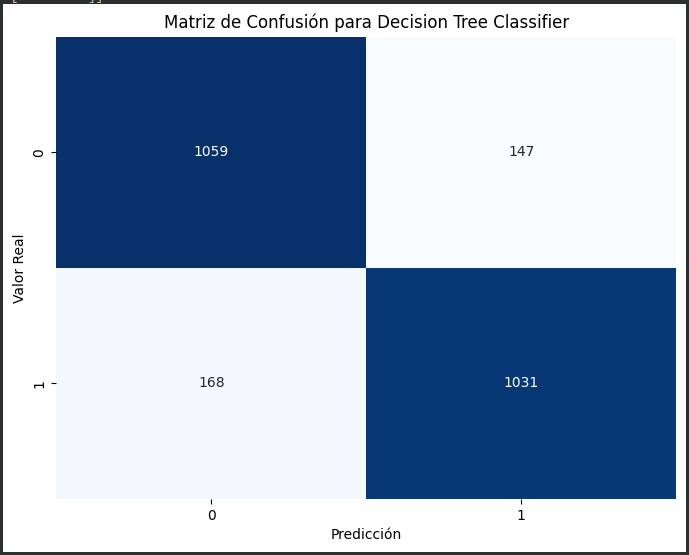
\includegraphics[scale = .4]{IMA/DecisionTreeMatriz.png}
\end{center}

\begin{itemize}
\item Verdaderos positivos (TP): 1059 (mensajes 'ham' clasificados correctamente como 'ham').
\item Falsos positivos (FP): 147 (mensajes 'spam' clasificados incorrectamente como 'ham').
\item Falsos negativos (FN): 168 (mensajes 'ham' clasificados incorrectamente como 'spam').
\item Verdaderos negativos (TN): 1031 (mensajes 'spam' clasificados correctamente como 'spam').
\end{itemize}
% ----------------------------------------------------------------------------------------\
% ---------------------------------------------------------------------------------------\
\subsection{Random Forest}
% ----------------------------------------------------------------------------------------\
% ---------------------------------------------------------------------------------------\

\subsubsection*{Métricas de evaluación}

\begin{itemize}
\item Precisión: el $93.18\%$ de los mensajes clasificados como 'ham' fueron realmente 'ham'.
\item Recall: el modelo obtuvo un $96\%$ correcto de todos los mensajes 'ham'.
\item F1-score: para ambas clases (ham y spam) se obtuvo un equilibrio del $93\%$.
\item Accuracy: La exactitud general del modelo es del $93\%$
\end{itemize}

\subsubsection*{Matriz de confusión}

\begin{center}    
    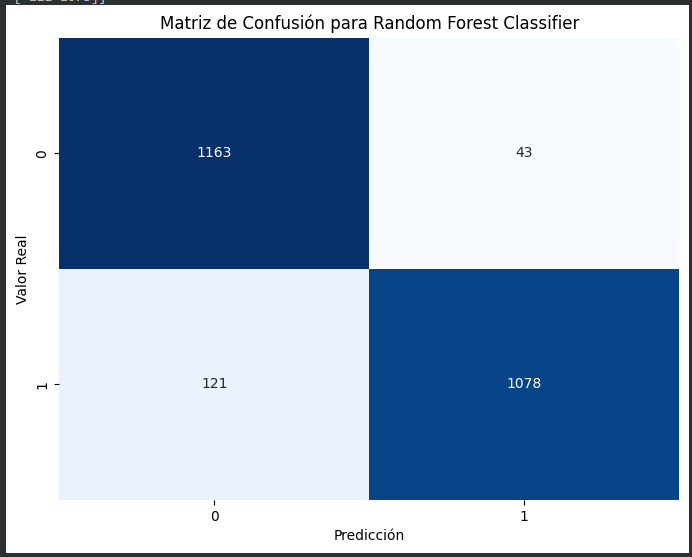
\includegraphics[scale = .4]{IMA/RandomForestMatriz.png}
\end{center}

\begin{itemize}
\item Verdaderos positivos (TP): 1163 (mensajes 'ham' clasificados correctamente como 'ham').
\item Falsos positivos (FP): 43 (mensajes 'spam' clasificados incorrectamente como 'ham').
\item Falsos negativos (FN): 121 (mensajes 'ham' clasificados incorrectamente como 'spam').
\item Verdaderos negativos (TN): 1078 (mensajes 'spam' clasificados correctamente como 'spam').
\end{itemize}